\documentclass[conference,comsoc,9pt]{IEEEtran}
\usepackage{listings}
\usepackage{color}
\usepackage{xspace}
\usepackage{graphicx}
\graphicspath{ {images/} }

\definecolor{mygreen}{rgb}{0,0.6,0}
\definecolor{mygray}{rgb}{0.5,0.5,0.5}
\definecolor{mymauve}{rgb}{0.58,0,0.82}

\lstset{
         basicstyle=\footnotesize\ttfamily, 
         numberstyle=\tiny,          
         numbersep=5pt,             
         tabsize=2,                
         extendedchars=true,      
         breaklines=true,        
         showspaces=false,      
         showtabs=false,       
         xleftmargin=17pt,
         framexleftmargin=17pt,
         framexrightmargin=5pt,
         framexbottommargin=4pt,
         showstringspaces=false,
         commentstyle=\color{mygreen},    % comment style
         keywordstyle=\color{blue},       % keyword style
         stringstyle=\color{mymauve},     % string literal style
 }

\def\sys{libFuzzer-bin\xspace}
\def\libfuzzer{libFuzzer\xspace}
\newcommand{\ttstyle}[1]{\texttt{\scriptsize #1}}

\begin{document}

\title{Design and Implement Binary Fuzzing\\based on \libfuzzer}
\author{
\IEEEauthorblockN{Wei-Chieh Chao$^1$, Si-Chen Lin$^1$, Yi-Hsien Chen$^1$, Chin-Wei Tien$^2$, Chun-Ying Huang$^1$}
\IEEEauthorblockA{$^1$ Department of Computer Science, College of Computer Science, National Chiao Tung University\\
$^2$ Cybersecurity Technology Institute, Institute for Information Industry}
}

\maketitle

\begin{abstract}
We design and implement \sys, a coverage-guided binary fuzzer based on \libfuzzer.
We discuss how \sys is implemented, measure the overheads of our implementation, and compare its performance against the American Fuzzy Lop (AFL) fuzzer.
This is a work-in-progress.
Our evaluation results show that, compared with the vanilla AFL, the current implementation brings only limited overheads and is able to identify possible vulnerabilities in a shorter time.
\end{abstract}


\section{Introduction}
\label{sec:intro}

  Fuzzing is a technique to automatically test software by providing random data as input. When fuzzing, we usually build a fuzzer to generate and send random inputs to the program. After program exit, it will send execution information back to the fuzzer. Then, the fuzzer will generate new input based on the execution information.

  When doing fuzz testing, we focus on crashes. That is, we try to generate input data that make program crashed. Therefore, fuzzer analyzes execution information such as path, coverage, and exceptions to decide what kind of input data is next time.

  American Fuzzy Lop (AFL)\cite{AFL} is one of the most famous fuzzing tools. There are two modes in AFL. One is source code mode, and the other is binary (QEMU) mode. Source code mode uses afl-gcc to compile the source code, in the meanwhile, it inserts lots of checkpoints to send execution information back. On the other hand, binary (QEMU) mode uses QEMU to run the binary, and it analyzes execution information from QEMU directly. Because of the implementation, it’s no doubt that source code mode would find crashes faster than binary (QEMU) mode.

  LibFuzzer\cite{libfuzz} is a library for coverage-guided fuzz testing. It only support source code mode. Different from AFL, LibFuzzer considers target source code as library, and it send inputs through “call function”. It compile its source code with target source code together.

  In some case, LibFuzzer found crashes much faster than AFL did. Heartbleed (CVE-2014-0160) was a critical security bug in the OpenSSL cryptography. It took couples of hours to find crash using AFL. However, it only took ten seconds to find crash using LibFuzzer. That’s one of the reasons that we wanted to build binary mode for LibFuzzer.

  Generally, we built a bridge for communication between LibFuzzer and binary. We used QEMU, as same as AFL, to generate runtime information. In detail, we executed binary through QEMU and analyzed runtime information from QEMU after exited. LibFuzzer need lots of information from binary, such as coverage, caller, and cmp. We focused on coverage here. Coverage is how many percent of codes have been executed. First, we used radare2 to generate basic blocks infromation. Moreover, we did static analysis before executing binary. Second, we executed binary through QEMU and analyzed runtime information dynamically. Finally, we sent coverage infromation back to LibFuzzer.

%
\section{Related Work}
\label{sec:related}



\section{Methodology}
\label{sec:method}

\subsection{Link IO together}

Normally, when using Libfuzzer, we put the source code need to be test inside \texttt{LLVMFuzzerTestOneInput} as describe in the introduction section.
But when we want to run a binary, we don't have source code.
Hence, what we do is actually putting \texttt{execv("our-binary", ..., ...)} inside the \texttt{LLVMFuzzerTestOneInput} to invoke our binary.
And before execute \texttt{execv} we need to use dup2 to link

\begin{enumerate}
  \item [1.] fuzzer test input $\to$ binary stdin.
  \item [2.] binary stdout $\to$ \texttt{/dev/null}.
  \item [3.] binary stderr $\to$ \texttt{/dev/null}
\end{enumerate}

The simplified code is something like below

\begin{lstlisting}[language = c++]
extern "C" int LLVMFuzzerTestOneInput(const uint8_t *Data, size_t Size) {

    int P_IN[2]; pipe(P_IN);
    if(Size) write(P_IN[1], Data, Size);
    ...
    int pid = fork();
    if(pid == 0) {
        dup2(P_IN[0], STDIN_FILENO);
        dup2(dev_null, STDOUT_FILENO);
        dup2(dev_null, STDERR_FILENO);
        ...
        execv(..., ..., ...);
    }
    ...
}
\end{lstlisting}

\subsection{Collect Runtime Information}

After we link IO together, the binary should get the input of the libfuzzer test input now.
Though it is runnable, Libufuzzer don't have any runtime information like code coverage and will stop running after a few rounds.
First, we need to figure out what Libfuzzer collect while running.
Libfuzzer collect runtime information through \textbf{Clang SanitizerCoverage}, which provides simple code coverage instrumentation and has hook function for customization.
Now we use qemu to collect right information for those hook function implemented by LibFuzzer.

\subsubsection{trace pc guard}




\section{Evaluation}
\label{sec:eval}

In this section, we will compare the performance of original LibFuzzer, our LibFuzzer and AFL. We use fuzzer-test-suite\cite{fuzzer-test-suite}, a set of tests for fuzzing engines provided by Google, as the test cases. In order to support our LibFuzzer, we modify the \texttt{target.cc} in some test cases. Take \texttt{c-ares-CVE-2016-5180} for example, we modified the \texttt{extern "C" int LLVMFuzzerTestOneInput(const uint8\_t *Data, size\_t Size)} function declaration to \texttt{int main()}. And use \texttt{read} function to read input data, the size is the length of input data. Check out more detail of patching fuzzer-test-suite in wiki page of our repository. The following specification is our machine information and all experiments were performed on it.

\begin{lstlisting}
virtual private server on Google Cloud Platform
n1-standard-1 (one vCPU, 3.75 GB RAM)
\end{lstlisting}

\subsection{Compared with original LibFuzzer}

We choose some CVE test cases in fuzzer-test-suite, including \texttt{CVE-2016-5180}, \texttt{CVE-2015-8317} and \texttt{HeartBleed (CVE-2014-0160)}, to evaluate the performance of our LibFuzzer. These are the output of running test cases by our LibFuzzer and do it 10 times to calculate the average time.

\begin{enumerate}
    \item [1.] \texttt{CVE-2016-5180}
\end{enumerate}

This is a 1-byte-write-heap-buffer-overflow in c-ares. This bug was one of out a chain of two bugs that made a ChromeOS exploit possible: code execution in guest mode across reboots.

\begin{lstlisting}
#0      READ units: 1
#2      INITED cov: 4 ft: 20 corp: 1/1b exec/s: 2 rss: 25Mb
#3      NEW    cov: 4 ft: 39 corp: 2/3b exec/s: 3 rss: 25Mb L: 2/2 MS: 1 CopyPart-
#4      pulse  cov: 4 ft: 59 corp: 2/3b exec/s: 2 rss: 25Mb
#4      NEW    cov: 4 ft: 59 corp: 3/5b exec/s: 2 rss: 25Mb L: 2/2 MS: 2 CopyPart-ShuffleBytes-
Error status : 139
Signal : Segmentation fault
\end{lstlisting}

And we can find the 1-byte-write-heap-buffer-overflow by our LibFuzzer within 3 seconds.

\begin{enumerate}
    \item [2.] \texttt{CVE-2015-8317}
\end{enumerate}

This is a 1-byte-read-heap-buffer-overflow and a memory leak in libxml2.

\begin{lstlisting}
#0      READ units: 1
Error status : 139
Signal : Segmentation fault
\end{lstlisting}

Using our LibFuzzer can find the 1-byte-read-heap-buffer-overflow and a memory leak within 120 seconds.

\begin{enumerate}
    \item [3.] \texttt{HeartBleed (CVE-2014-0160)}
\end{enumerate}

This is a multi-byte-read-heap-buffer-overflow in openssl.

\begin{lstlisting}
#0      READ units: 1
...
Error status : 134
Signal : Aborted
\end{lstlisting}

In this test case, we cannot find the multi-byte-read-heap-buffer-overflow because this is a network service and there are a few asserts cannot pass by running program in local. As a result, we only got an aborted signal not segmentation fault.

Compared with original LibFuzzer and plot the chart.

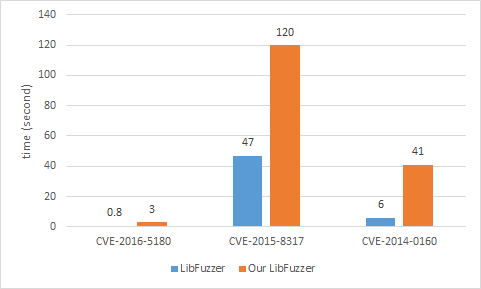
\includegraphics[width=\linewidth]{eval1.png}

As we can see, because the implementaion of our LibFuzzer, the IO speed and analysis take a lot of time. And the preformance is slower than original LibFuzzer. But compared the time of original LibFuzzer and our LibFuzzer took, we still can find the bugs efficiently in these test cases.

\subsection{Compared with AFL}

According to the section of binary-only instrumentation in the technical whitepaper for afl-fuzz, we know the overhead of the QEMU mode is roughly 2-5x. So we try to compare with the overhead, the time of linking IO and analyzing the output, between AFL and our LibFuzzer. And the following chart is the overhead of the test cases we ran before.

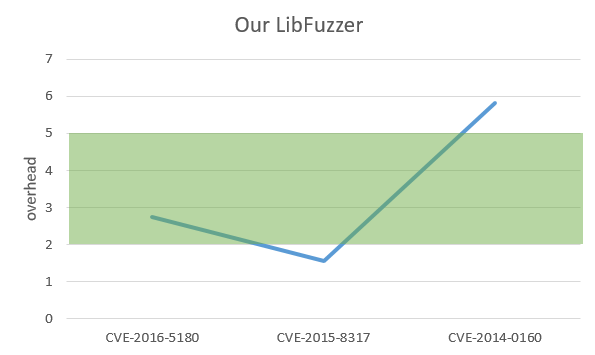
\includegraphics[width=\linewidth]{eval2.png}

The green area is the overhead of the QEMU mode and the bule line is our LibFuzzer overhead. We can see the result is close to the QEMU mode and therefore it maybe cost that much time to do analyze and link IO for supporting binary only mode.



\section{Conclusion}
\label{sec:conclusion}



\bibliographystyle{IEEEtran}
\bibliography{libfuzz}

\end{document}

